\chapter{Conception de la solution}

\section{Modélisation C4}
Dans le cadre de la conception et de la documentation des architectures logicielles, il est impératif de disposer de méthodes claires et structurées pour représenter les différents aspects du système. La méthode de modélisation C4 (Context, Container, Component, Code), développée par Simon Brown, répond à ce besoin en fournissant un ensemble de diagrammes permettant de capturer et de communiquer efficacement l'architecture d'un système logiciel à différents niveaux de détail. \\

\noindent La méthode C4 se distingue par son approche hiérarchique et progressive, qui permet de passer d'une vue d'ensemble du système à une vue détaillée des composants individuels. Elle se compose de quatre niveaux de diagrammes: \\

\begin{itemize}
    \item \textbf{Diagramme de contexte}: ils montrent le système dans son environnement, incluant ses relations avec les utilisateurs et d'autres systèmes;
    \item \textbf{Diagramme de conteneurs}: ils illustrent la décomposition du système en conteneurs interdépendants, chaque conteneur étant un sous-système exécutable déployable indépendamment;
    \item \textbf{Diagramme de composants}: ils détaillent la décomposition des conteneurs en composants interdépendants et, si nécessaire, leurs liens avec d'autres conteneurs ou systèmes;
    \item \textbf{Diagramme de code}: ils fournissent des détails supplémentaires sur la conception des éléments architecturaux, souvent en utilisant des notations existantes comme UML, des modèles entité-association ou des diagrammes générés par des environnements de développement intégrés (IDE). \\
\end{itemize}

\clearpage

\section{Diagramme de contexte}

Le diagramme de contexte est une représentation visuelle des interactions entre un système et son environnement. Au centre du diagramme se trouve le système lui-même, représenté par un bloc, entouré par des acteurs externes ou des systèmes avec lesquels il interagit. Ces acteurs externes peuvent être des personnes, des organisations, des systèmes informatiques, etc. Les interactions entre le système central et les acteurs externes sont généralement représentées par des flèches indiquant le flux d'informations, de données ou de contrôle entre eux. \\

\noindent La solution d'automatisation du registre de traitement

\begin{figure}[H]
    \centering
    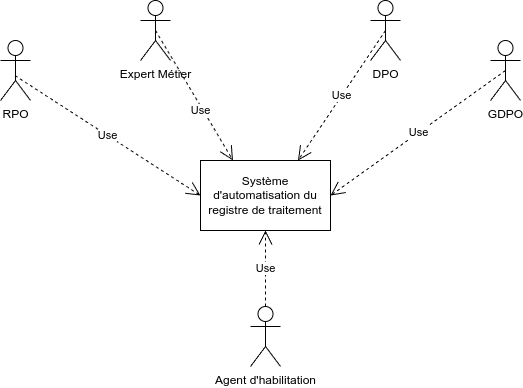
\includegraphics[width=.8\textwidth]{images/context-diagram.drawio.png} \\[.4cm]
    \caption{Diagramme de contexte}
\end{figure}


\clearpage

\section{Diagramme de conteneurs}

\noindent Le diagramme des conteneurs de la solution d'automatisation du registre de traitement comprend trois éléments principaux :


\begin{itemize}
    \item \textbf{Application web monopage (SPA)} : Permet aux utilisateurs d'interagir avec les fonctionnalités sans rechargement de page. Gère la visualisation, la saisie et la modification des données;
    \item \textbf{Serveur d'API}: Traite les requêtes HTTP de l'application web. Gère la logique métier, la validation des données, et la gestion des utilisateurs et des autorisations;
    \item \textbf{Base de données}: Stocke de manière sécurisée toutes les données de l'application. Assure la persistance et la sécurité des données, incluant les fiches de traitement, les informations sur les utilisateurs et les journaux d'activité. \\
\end{itemize}




\begin{figure}[H]
    \centering
    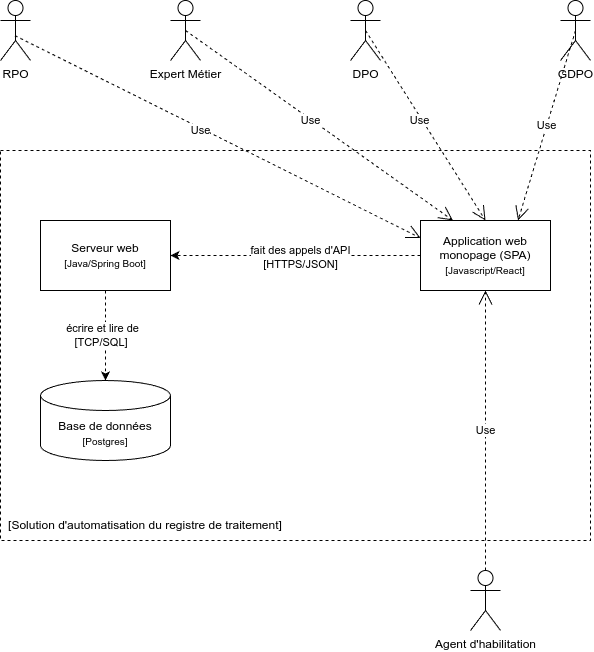
\includegraphics[width=.85\textwidth]{images/container-diagram.png}
    \caption{Diagramme de conteneurs}
\end{figure}

\clearpage


\section{Diagramme des composants du serveur web}

\begin{figure}[H]
    \centering
    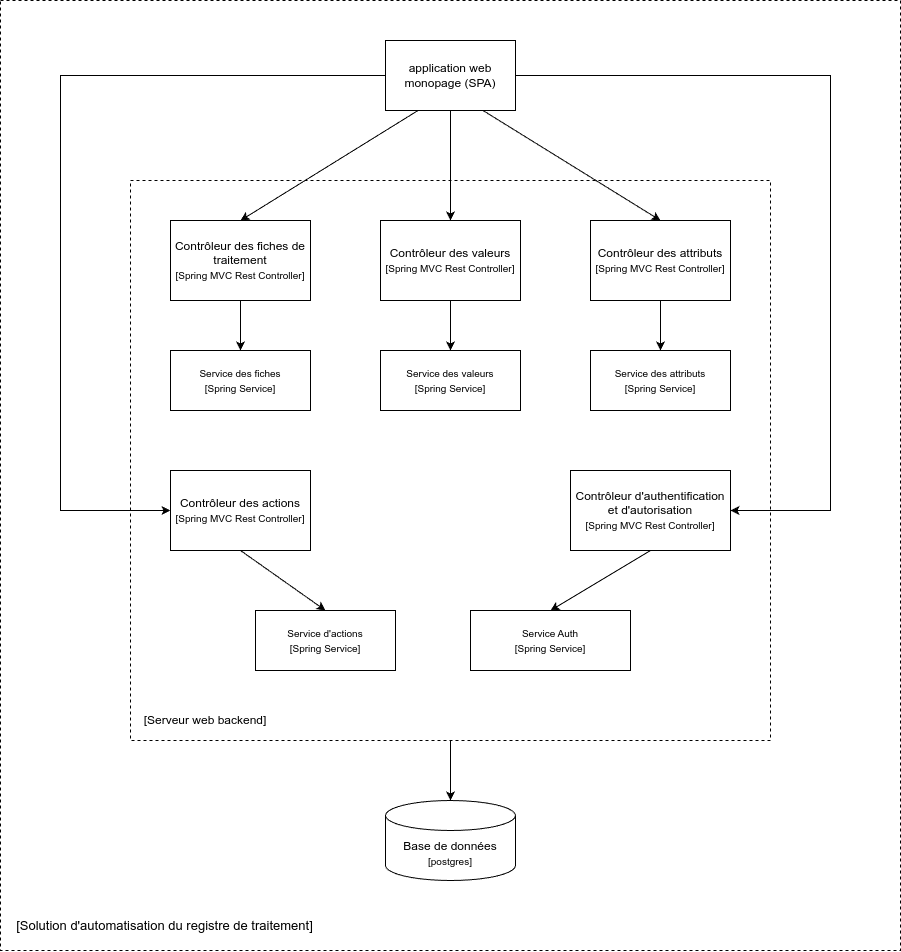
\includegraphics[width=\textwidth]{images/component-diagram.png}
    \caption{Diagramme des composants}
\end{figure}



\clearpage
\section{Diagrammes de classes du serveur d'API}


\subsection{Couche modèle}
\begin{figure}[H]
    \centering
    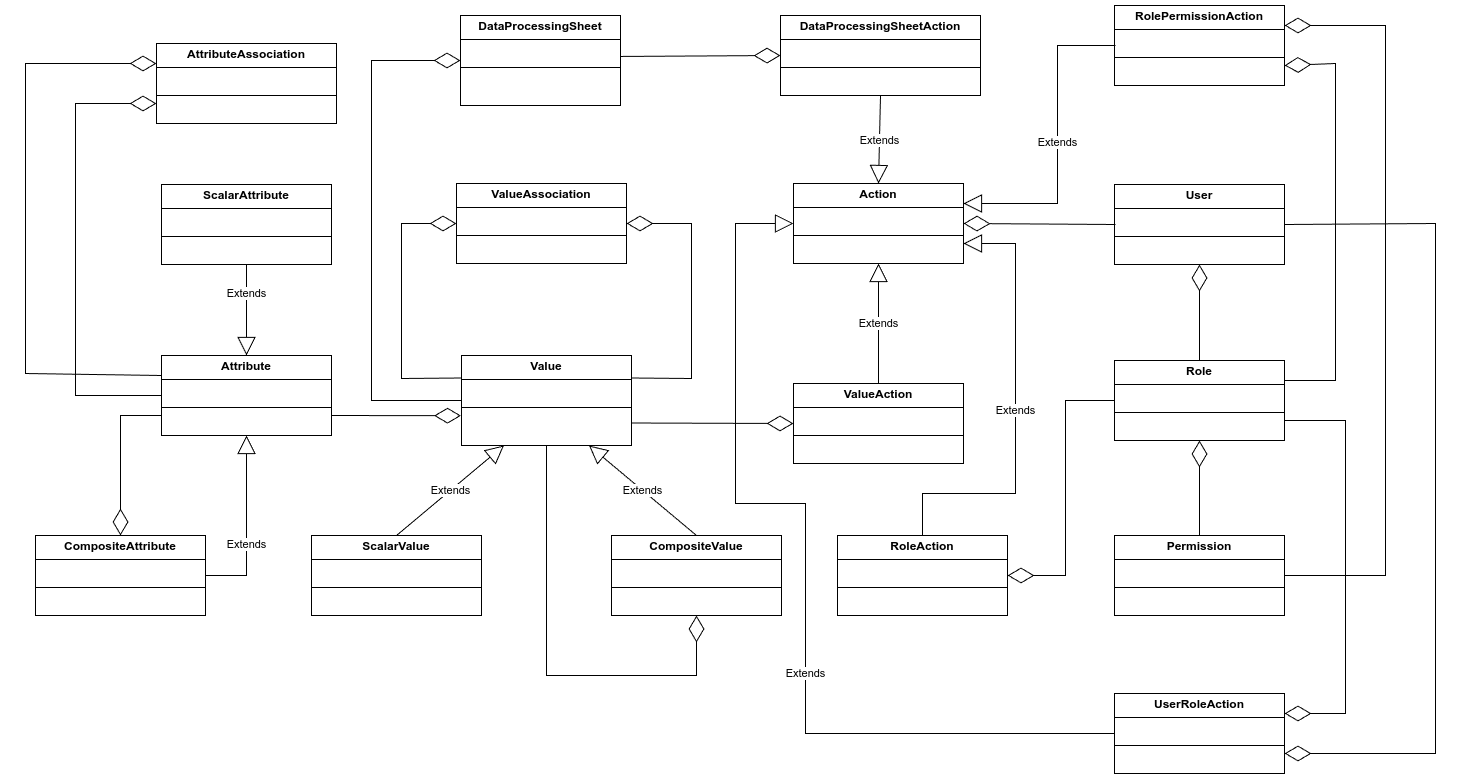
\includegraphics[height=.75\textwidth, angle=90]{images/class-diagram.png}    
\end{figure}


\section{Diagrammes de séquences}

\subsection{Ajout d'un paramètrage}

\vspace{.2cm}

\begin{figure}[H]
    \centering
    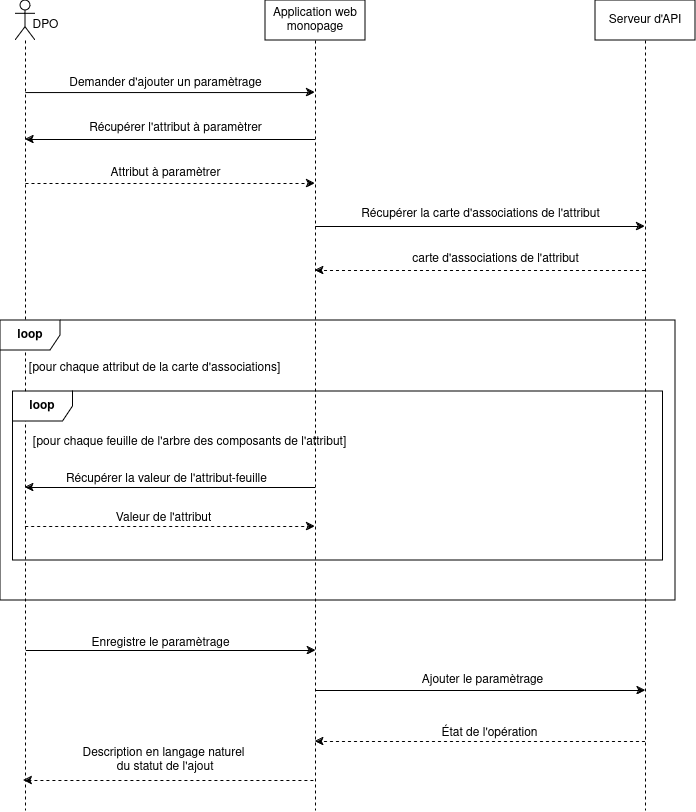
\includegraphics[width=\textwidth]{images/sequence-diagram-value-creation.png}
\end{figure}